\documentclass[11pt, twocolumn]{article}


% \IEEEoverridecommandlockouts               % This command is only needed if
%                                            % you want to use the \thanks command

% \overrideIEEEmargins                     % Needed to meet printer requirements.

\usepackage[style=ieee]{biblatex}
\usepackage{amsmath}
\usepackage{graphicx}
\usepackage{fullpage}
\usepackage{subcaption}
\usepackage{url}
\usepackage{csquotes}
\usepackage[american]{babel}


% \DeclareMathOperator{\atantwo}{atan2}

% \DeclareMathOperator{\arctantwo}{arctan2}

%\setlength{\belowcaptionskip}{-6pt}
\setlength{\textfloatsep}{8pt}

\newcommand{\parallelsum}{\mathbin{\!/\mkern-5mu/\!}}


\DeclareMathOperator{\atantwo}{atan2}

\DeclareMathOperator{\arctantwo}{arctan2}

\addbibresource{abrv.bib}
\addbibresource{refs-chains.bib}
\addbibresource{djbref.bib}
\addbibresource{swarm.bib}



\title{The best peg-and-hole joint}
\author{Weifu Wang \and Devin Balkcom}


\newcommand{\bo}{\mathbf o}
\newcommand{\bq}{\mathbf q}
\newcommand{\bp}{\mathbf p}
\newcommand{\bd}{\mathbf d}
\newcommand{\bn}{\mathbf n}
\newcommand{\bc}{\mathbf c}

\begin{document}
\maketitle

\begin{abstract}
In this work, we explore how to design a good peg-in-hole joint that can be most stable even when error occurs in both the manufacturing and the assembly stages. Without error, a peg-in-hole joint can be designed with ease, usually with edge-edge contacts along the boundary of the hole. In reality, error can affect these edge-edge contacts in different ways. Manufacturing error can change edge-edge contacts to point-edge contacts at different and unpredictable locations, thus reducing the stability of the entire joint. The manipulation error can also change edge-edge contacts to point-edge contacts in an unpredictable fashion. We will explore the design of peg-in-hole joint with point-edge contact in mind, so that manufacturing error and manipulation error does not change the mode of the contacts. We will also explore how can the contacts be designed so that even under manufacturing and manipulation error, the points on the peg that suppose to make contact with the hole still maintain contact, and provides as much stability to the assembly as possible. 
\end{abstract}

\section{Introduction}

Joinery based assembly is where between the building blocks, external binder like cement or glue is not used so that the blocks of assembly is attached to each other by the joints that are built into the building blocks. Reversible is a key feature in joinery based assembly. 

However, because the joinery based assembly process is reversible, the joints that are assembled together should not be locked by friction, but supported by geometry and normal forces. Such requirements imposes many constraint on the joints. Apart from the precision of the manufacturing process, the contacts between the joints and the forces they impose on each other have to be planned during the design stage. 

Traditionally, edge-edge (face-face) contacts are adapted in the assembly to provide sufficient contact area to provide stability. Such strategy can be problematic as surface contacts may impose friction lock between joints, and is highly sensitive to errors. Traditional assembly avoids such problem by applying deformable glue between surface contacts. 

Different errors arise in the assembly process. Manufacturing error is a major source of error as expected, which is also unavoidable. Even though modern manufacturing process has advanced to a stage where the error can be very small compared to the size of the block or joint. However, even such small error would pose big challenge in the joinery based assembly as these errors can change the contact mode from surface contacts to point-surface contact. Such change would mostly invalid the overall design of the joints. 

In the assembly process, especially when we would like to use robots to implement the assembly process automatically, errors also appear as even the state-of-the-art robots are not perfect in precision and they are not equipped with adaptability that can reduce sensing and manipulation error during the assembly process. Such errors can also change the contact mode between joints and blocks, leading to unpredictable contact locations and assembly outcomes, either making the upcoming assembly difficult and unstable, or leading to an unacceptable final assembly outcome. 

In this work, we explore the design of the joints that can lead to predictable and (reasonably) stable assembly even when errors from different sources occur. Instead of the surface contacts, we design the joints to make contacts at a collection of points. By making these points be the planed contacts, the small errors in the manufacturing process should change the location of these points in the minimal fashion so that the contact locations are still predictable. What is more, we also plan these contacts at locations such that when assembled, even under arbitrary external forces, the contacts should remain in place or change minimally to provide the most stability. Also with point contacts, the assembly process can also be tolerant to errors as the edges joining the planned contact points can be designed to have the desired slant or curvature to lead the contacts into their desired contact locations, rather than being locked by geometry or friction that can prevent the joints from moving to the desired locations. In this paper, we focus on the peg-in-hole type of joint as a start, and we will move to other types of joints that are used in the joinery assembly. 

The paper organizes as follows, we will first introduce the joint design if no manufacturing error is present, and show the stability analysis and limitations (Section~\ref{sec:perfect}). Then, we will show how to change the design to cope with errors from different sources (Section~\ref{sec:with_errors}). Based on the analysis, we conduct experiments to show the validity of the design and analysis (Section~\ref{sec:exp}). Finally, we conclude the work by presenting the future directions. 



\section{Related work}



%Fold-able origami robots. Modular robots in general. Closed chain kinematics.

% swarms, flocks, crowds

Linearizing motion around an initial configuration allows study of systems of blocks with many thousand degrees of freedom; our approach draws inspiration from early work on {\em manipulability ellipsoids}~\cite{Chiacchio1991-manipulability,Park1998-manipulability,Kim1998-manipulability,Bicchi2000-manipulability}, in which directions of motion of the end effector of a robot arm are analyzed at a particular configuration by examining eigenvectors of the Jacobian matrix. Work by Berenson also provides analysis and approximations of Jacobians for truly flexible cloth or string~\cite{Berenson2013-deformable}. Linear grasp analysis techniques also serve as inspiration. In the 19th century, Reuleaux~\cite{Reuleaux1876} derived a geometric method to find the free motion of an object in contact with frictionless fingers. Mishra, Schwartz, and Sharir's seminal work on the minimum number and sufficient placement of fingers to immobilize an object~\cite{Mishra1987-grasp-existence} analyzes polyhedral constraints in twist and wrench spaces.

In contrast to manipulability and grasping problems, the blocks which we consider are only loosely connected. Caging grasps~\cite{RodriguezMF12,makita2008,vahedi2008caging,erickson2003capturing,rimon1996caging,allen2015two,Makita2017-caging-survey} study how robot hands may loosely capture an object; the present paper studies motion of structures in which either pairs of blocks or combinations of many blocks may cage each other. Direct construction of configuration spaces of pairs of blocks has a long history; Sacks {\em et al.}~\cite{SacksBM17} provides a recent approach, and gives a much higher-fidelity representation of the free motions of small numbers of blocks than our edge/point distance function model. Eckstein {\em et al.}~\cite{Eckenstein2017-acceptance-area-connectors} analyze how forgiving a connector design is using an explicit approximation of the configuration space of the joint.

The Carpenter's Rule Theorem states that any open polygonal chain (a planar revolute robot arm) can be reconfigured arbitrarily without self-intersection~\cite{Connelly2003-carpenters}; the proof uses {\em expansive motions} that cause points and edges to separate from one another. The motions in the present paper allow points and edges to approach one another, while balancing the rates so as to optimize net motion in some direction. The distance constraints are similar to those used in Linear Complementarity Problem (LCP) formulations of dynamics~\cite{STsiam97,TTPrs01}, which have been used both for rigid body simulation and design for manipulation~\cite{Balkcom2002b}.

Tolerance analysis of mechanical assemblies is utilized in mechanical engineering to determine how frequently small manufacturing errors in the component parts of an assembly will result in unacceptable deviations in the final assembly~\cite{Chase1991-survey-of-tolerance-analysis}. The Direct Linearization Method~\cite{Chase1996-geometric-tolerance-analysis} linearizes the homogeneous transformation matrices describing the kinematics of an assembly, and applies statistical techniques to determine what percentage of assemblies are able to be assembled.
% djb: a bit verbose
%The goal of tolerance analysis is to aid the engineer in designing mechanical assemblies which are robust to a distribution of possible manufacturing errors commonly seen in mass manufacturing


%This work is similar to ours in that it utilizes a linear approximation of the nonlinear configuration space of an assembly, but the focus is to predict how often assembly closure requirements are met given a distribution of errors. Like our work, the linearization is used because the relative motion between components is small.



Methods for building modular interlocking structures have been studied by Zhang {\em et al.}~\cite{Zhang2018-interlocking,Zhang2016a} and by Werfel {\em et al.}~\cite{Werfel2006-mobile-robot-construction}; however, the structures are assumed to be static after construction with idealized perfect connectors between blocks. Techniques for robot swarm control typically must handle thousands of simple robots collectively performing some tasks, e.g., object transports~\cite{alonso2017multi}, shape generation~\cite{hsieh2008decentralized}, self-assembly~\cite{o2014self,rubenstein2014programmable}, and network connectivity~\cite{esposito2006maintaining}; perhaps the closest work in spirit to the present is~\cite{ShahrokhiMB17}, which controls swarms of robots by allowing robots to bounce off of non-slip walls.


%While the distributed approach frequently taken to swarm control has both computational and implementation advantages, we note that the present work's linear constraint approach allows interesting interactions between the rigid bodies

\section{Ideal joint subject to no manufacturing error}
\label{sec:perfect}

When the physical block is in the exact shape we designed, assembly can be simple. However, in reality, it is not always the case. That being said, the current manufacturing technology can produce blocks that are basically the same as what we designed with little error. So, the desired condition when no error exists can provide a base for the design that can tolerate errors. 

In this work, we focus on the peg-in-hole joint, which we assume to be symmetric along both $x$ and $y$ axes. Therefore, we start by investigating the planar case of the peg-in-hole joint. The assumption is not outrageous because if the basic shape of the block is a cube, then the assembly of the blocks are aligned along the $x$ and $y$ axes. Therefore, little to none rotation around $z$ axis should be introduced to the blocks and joints during assembly. As we will show, the planed contacts are between points on the peg and surface on the boundary of the hole, the small error in orientation will not violate the analysis in the plane. 


\subsection{Ideal joint for stability}

Once the peg is successfully inserted into the hole, we need the peg to be stable, i.e. be able to withstand a large variety of external forces, which occurs naturally during the assembly. One of the major issue in our previous block assembly experiments is the inserted joints rock inside the hole joint during assembly, which in turn creates further error in the later assembly. Surface contacts and unpredictable contact locations is the main cause for the rocking in the previous experiments. 

We will explore the possibility of point-surface contact rather than direct surface-surface contact. By switching to point contact from surface contacts, we can not only predict the contact locations, even under limited errors, but we can also analyze how these contacts can change under external forces as the locations of them are known. 

A first intuition would be that the more contacts there are, the more stable the peg would be inside the hole. However, the more contacts there are, the more it would suffer from imperfection in the manufacturing process, as it would be difficult to predict how the contacts will shift as the error occurs, so we cannot rely on the number of contacts to provide stability. 

On the other hand, if there are only a few contact points between the peg and the hole, even though the imperfection in the manufacturing process can still affect those contact points, the resulting contact points would still be on or nearby the selected points if the difference between the contacting points and the rest of the peg is large enough to overcome the manufacturing error. Therefore, the placement of these selected few contact points would become critical. 

For stability, a minimum of three contact points should be selected. What is more, considering that the hole is symmetric as well as the peg, the contacts should be symmetric in order to provide force closer. Extending from the concept of immobilizing planar objects, at most six contacts would be needed for the immobilization and force closer. So, how many should we select and where to place them? 

\begin{figure}
\begin{center}
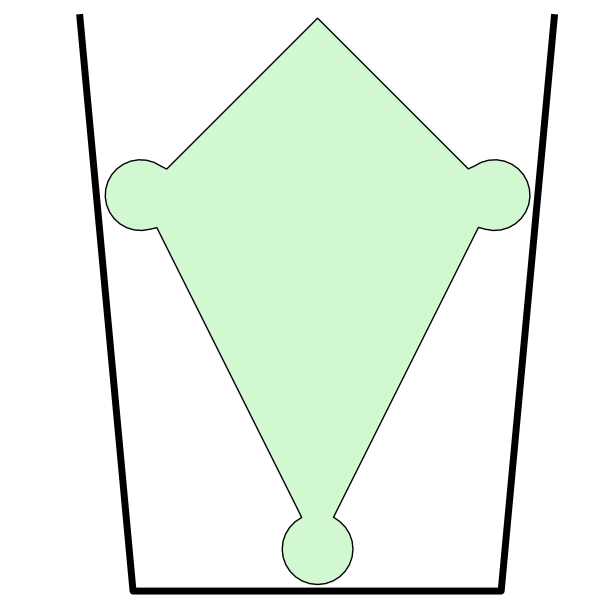
\includegraphics[width=1.5in]{figures/three_contact.png}
\end{center}
\caption{Peg making three contacts with the hole joint. If no error exists, these three contacts is sufficient to provide stability. }
\label{fig:three_contact}
\end{figure}


When all errors are excluded, three contacts are sufficient to provide the peg stability inside the hole joint, as shown in Figure~\ref{fig:three_contact}. As no error exist, the peg cannot translate horizontally inside the hole, but only vertically up to exist the hole. Rotation of the peg, however, is not impossible geometrically. If we consider an outward pointing normal at each contact point between the peg and the hole, then a possible rotation of the peg would be that all contact points {\em slides} to the left of the original normal. 

To prevent such a rotation, we need to make sure that if any two contact slides along the surface of the hole joint, the third contact would create a {\em pinch} situation. Because the bottom contact cannot get into a pinch situation, we will need to make sure the side contacts would create a pinch situation when sliding. Since the peg is symmetric, we can only consider one contact. Let us consider the previously mentioned sliding direction, all towards the left of the original contact normal. 

Let the radius of the bump be $r$, the distance between the two centers of the side bumps be $2d$, and the midpoint  of the line connecting two side bump centers have distance $h$ to the center of the bottom bump center, and let that midpoint be the origin $(0, 0)$. Also, let the side of the hole slant at an angle of $\alpha$. Let us denote the rotation angle of the peg by $\beta$, the orientation difference between the center axis of the peg before and after rotation. 

If the sliding is possible and the peg rotates an angle $\beta$, let the new coordinate of the previous origin be $(x, y)$, we will have, 

\begin{eqnarray}
|y| = h(1 - \cos\beta)\\
\tan\alpha = \frac{d}{h}
\end{eqnarray}
which indicates that as long as $\alpha < \arctan(\frac{d}{h})$, the pinch will happen, so the rotation of the peg is not possible inside the hole. 

However, if there exist an external force that have a projection that is along the axis of the peg pointing outwards of the hole joint, it is still possible to move the peg inside the hole. The contacts may depart from the surface, making the peg only contacting the hole at one point or even not contacting at all. We will not consider such situations since the peg-and-hole joint can never prevent such situations as there is no balancing force along the extraction direction. 

Another important design measure of the peg joint is the length of the peg versus the width of the peg. Based on the previous analysis, even though as long as the slant of the hole satisfy the condition, the pinch can prevent peg of any rotation, this ratio can potentially affect how robust of those contacts against external forces. By robust, we mean the size of the wrench cone that can change the contacts to get into the pinch condition. If the peg and the hole are both perfectly rigid, the pinch should be able to prevent all potential forces, but in reality nothing is perfectly rigid. Therefore, the less we rely on the pinch to prevent rotation, the more stable the peg will be inside the hole. 

Using the method introduced in~\cite{} to analyze the size of the wrench cone that can change contact modes, we can analyze the robustness of those contacts. Given the three contacts at the defined locations, the analysis show that when there is no error, the shorter the peg is, the more robust the contact will be, i.e. the smaller the wrench cone is that can move the peg contact points. 

The result is not hard to interpret. The shorter the peg is, when a force try to rotate it, the less the side contact location will rotate, thus the more overlap it has with the original contact point, i.e. the original contact location serves as the pinch contacts. As the peg becomes longer, a small rotation of the peg will move the original contact location by a large amount, thus the original contact is no longer part of the pinch configuration. Therefore, the shorter the peg is, under perfect condition, the more robust the contacts are to external forces. 

A shorter peg also means that the slant of the hole can be larger without giving up the pinch condition. The more gentle the slant is, the easier it is for insertion, which we will discuss in the next section. 



\subsection{Ideal joint for insertion}

Inserting a peg in a hole is not easy when implemented by a robot. A slight change of the orientation of the insertion can get the peg stuck along the edge of the hole, and keep applying forces along the tip of the peg will not be able to {\em unstuck} the peg. This is especially challenging when the contacts designed between the peg and hole are surface contacts. Therefore, sharp corners of the peg will easily get into a pinch situation with the edge of the hole. A slight offset perpendicular to the depth of the hole can also introduce problems, and surface contacts in this situation is again not beneficial. 

To overcome the pinch situation to allow the tip of the peg into the hole, the edge of the hole should be vertical or even be tilted so that the bottom of the hole is wider. On the other hand, to overcome the issue with the offset perpendicular to the depth of the hole, the edge of the hole should be tilted so that the entrance should be wider. Obviously, these two conditions are contradictory, so what should be the ideal design of the hole to allow this easy insertion? 


Many of the above issues are caused by the surface-surface contacts and sharp corners. Since we have decided to adapt point contacts rather than surface contacts, the analysis becomes simpler. A slanted edge of the hole can address most of the issues. The key would be how much slant can there be. 

Geometrical stability dedicates that the slant cannot be more than $\arctan{\frac{d}{h}}$. To avoid insertion pinch, the slant should be smaller, while to avoid the translational offset, the slant should be larger. Question is, given the slant angle no larger than $\arctan{\frac{d}{h}}$, and the point contact design shown above, can the insertion pinch still happen? Let us assume that the insertion angle cannot be larger than $\theta$, and the translational offset cannot be larger than $\Delta$. In addition, let the friction coefficient between the peg and the hole be $\mu$. 

To analyze the potential pinching situations, the translational offset can be dropped, as long as the slant of the side of the hole joint is consistent, which we will assume to be the case here. Based on the shape of the peg designed above, in order for a pinch-like condition to happen, the circular bump at the tip of the peg will need to be contacting the side of the hole while the other side of the hole will contact one of its side bump-contacts, as shown in Figure~\ref{fig:tilt}. 

\begin{figure}
\begin{center}
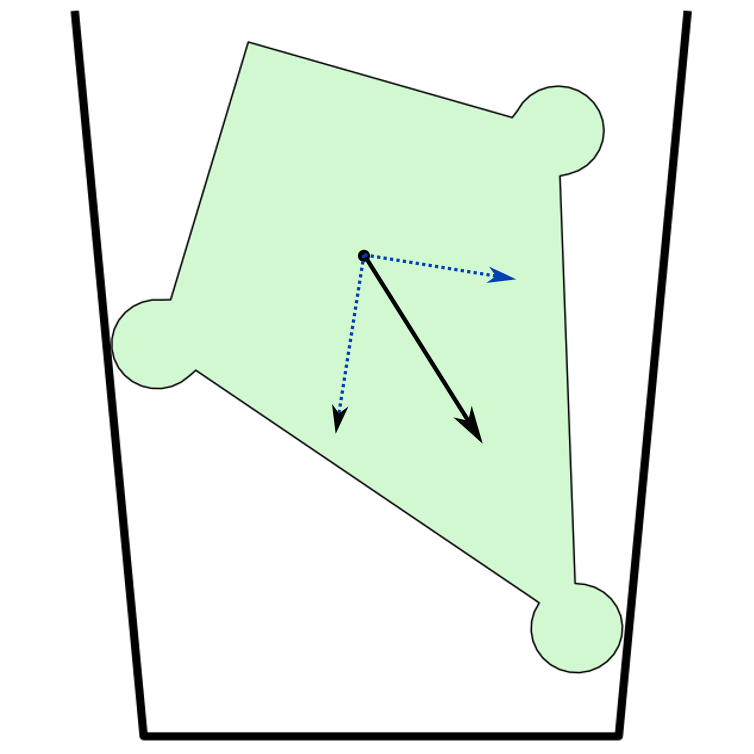
\includegraphics[width=1.5in]{figures/tilt.png}
\end{center}
\caption{Peg inserting into the hole with a small rotation angle of $\theta$. The tip of the peg contacts the side of the hole. }
\label{fig:tilt}
\end{figure}

So, in order for the peg to be able to continue moving towards the bottom of the hole joint, we will need to have $F\cos{\frac{\pi}{2}-\theta-\alpha}\cdot\mu \leq F\sin{\frac{\pi}{2}-\theta-\alpha}$, which lead to $\theta+\alpha\leq \arctan{\frac{1}{\mu}}$. Therefore, as long as the total tilting angle is not too large, the peg should be able to continue the insertion. 

In the illustrated insertion situation, when the condition of the total tilting angle is bounded as shown above, even when the hole becomes narrower so that the peg can no longer move deeper into the hole without rotation, because the force projection along the depth of the hole is larger than the friction between the peg and the hole, the force is sufficient to push the peg to rotate, reaching the bottom of the hole. 

\begin{figure}
\begin{center}
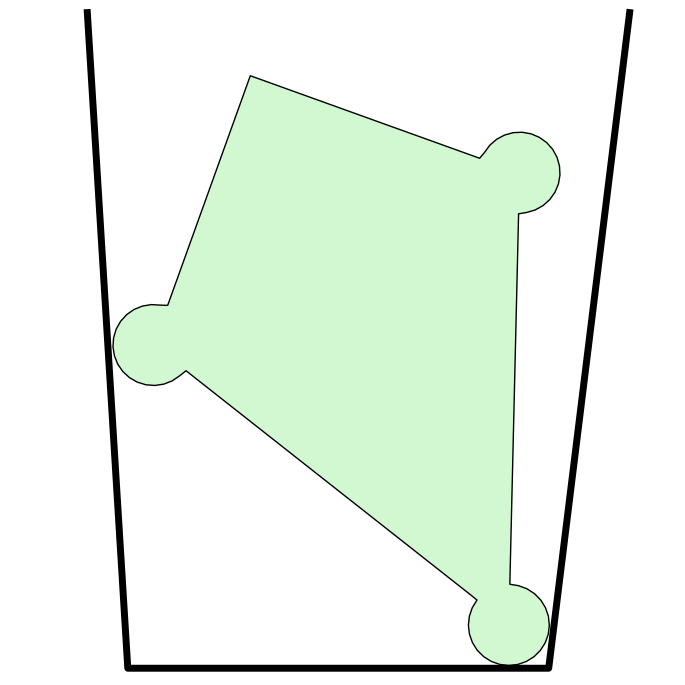
\includegraphics[width=1.5in]{figures/contact_bottom.png}
\end{center}
\caption{Peg inserting into the hole with a small rotation angle. The tip of the peg contacts both the bottom and side of the hole. }
\label{fig:contact_bottom}
\end{figure}

Another problem rises though, based on the design shown above. When the tip of the peg keep sliding towards the bottom of the hole, once it contacts the bottom of the hole joint, as well as the right side of the hole joint (Figure~\ref{fig:contact_bottom}), the force pushing the peg may not be able to adjust the peg into the desired configuration as shown in Figure~\ref{fig:three_contact}. Such situation cannot be resolved unless an adjustment of insertion force is made, mainly, the direction of the force. This would also suggest that if there do exist a small error in the insertion angle, based on the three contact design, the  peg cannot reach the desired goal configuration, which suggests that our design needs to be modified. 

\begin{figure}
\begin{center}
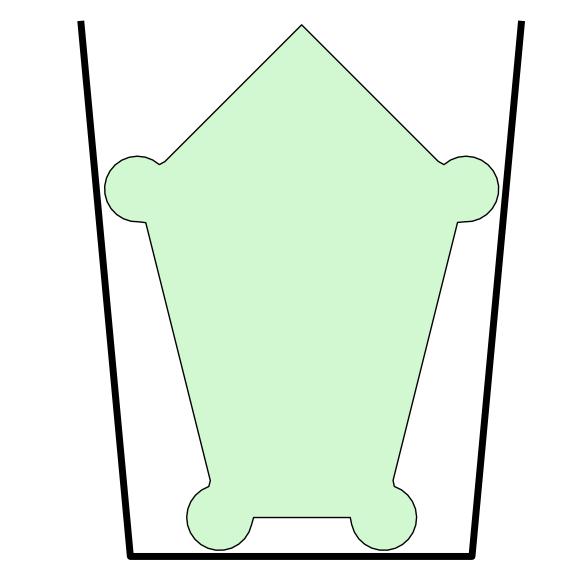
\includegraphics[width=1.5in]{figures/four_contact.png}
\end{center}
\caption{A redesigned peg, with four contacts in total. Two contacts at the sides of the peg, and two at the tip of the peg. }
\label{fig:four_contact}
\end{figure}

The key is to avoid the situation where a single desired contact point, which has to be modeled as a circular bump on the peg, can contact two sides of the hole at the same time. Therefore, a single bump at the tip of the peg cannot be used, but a set of two contacts at the tip of the peg can successfully avoid the situation stated above, as shown in Figure~\ref{fig:four_contact}. Based on the width of the the two contacts at the tip of the peg relative to the width of the hole, the force pushing the peg into the hole can make the transition between the contact of the tip with the side of the hole, to the contact between the upper-right contact with the side of the hole. 

Let the distance between the two tip contacts be $2w$, and recall that the depth of the peg is denoted as $H$, then the angle constraint becomes $\theta+\alpha+\arctan{\frac{w}{h}} \leq \arctan{\frac{1}{\mu}}$. The larger the distance between the two contacts on the tip, the smaller the total tilt angle can be, so we may not wish to have the distance between the two tip contacts be too large. 

On the other hand, the smaller the distance between the two tip contacts, the harder it is to transition from the tip contacts to side contacts with the hole, as the limit of that is the single contact at the tip, which can contact both the bottom and the side of the hole and can never transition to the side contacts on the peg. 

Because of the two contact near the tip, the goal is to never let the designed bump to make contact with two edges at once, i.e. maintaining the point contact design. But since the bump have a non-zero radius, it is always physically possible to have a small but none-zero tilt of the peg, and both contacts near the tip contacts the bottom of the hole, while one of the bump still makes contact with the side of the hole. Therefore, we need to have the bumps to have very small radius as a first constraint. Second, at the time or before the above stated situation happens, we would like to have the contacts shifted from the tip contacts to the side contacts. This leads to a relative small distance between the tip contacts, where as the tilt of the peg reduces due to the pushing of the peg into the hole, the peg can make both contacts at the side of the hole, and further push of the peg into the hole will separate the tip contact with the side wall of the hole, as shown in Figure~\ref{fig:four_contact_tilt}. 

\begin{figure}
\begin{center}
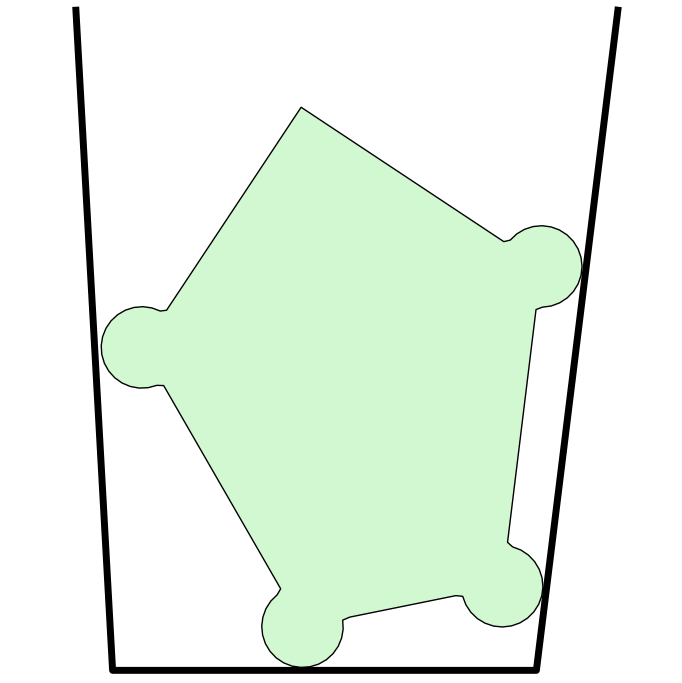
\includegraphics[width=1.5in]{figures/four_contact_tilt.png}
\end{center}
\caption{A tilt of the peg makes four contacts with the hole, but not yet at the desired locations. But on the side of the wall, the peg makes two contacts with the side of the hole, and further push of the peg will separate the contact between the bottom-right tip of the peg with the side of the hole. }
\label{fig:four_contact_tilt}
\end{figure}

Now, putting the above analysis together. When there are no manufacturing errors, to allow successful insertions as well as stability after insertion, we should have four contacts designed with the peg, two near the tip, two on the side. 


\section{Joint design subject to manufacturing error}
\label{sec:with_errors}

% uniform error

The problems rises when manufacturing error starts to be introduced. A few assumptions needs to be made before we go any further. First, let the peg and the hole both be attached to a wide block, so that when peg is fully inserted inside the hole, the edges will make contact. Second, let the error only occurs on the peg and let the hole be unchanged. Third, let the errors be uniform everywhere on the peg and the error reduces the size of the peg. 

The first assumption is placed to simulate real assembly scenarios. The second assumption allow us to analyze the change of contacts and how the peg can be moved inside the hole relatively. The third assumption is reasonable because usually the blocks can be made with molds, and exceeding the allowed size is impossible. 

With the given assumptions, we will show how to place the contacts to best reduce uncertainties and remain stable, both during insertion stage and after insertion. 


\subsection{Potential shift of contacts}

When the peg is off by $\epsilon$ in the production, it is also shorter from the base to the tip. Therefore, given the hole to be the same depth, and the existence of the external block, the originally planned contacts near the tip of the peg can no longer make contact, and on the side, at most one point can make contact due to the uniform reduction of width from the production error. This provides opportunity for rocking, and the peg is obviously not stable inside the hole. 

If the uniform error $\epsilon$ exists, first we need to recognize that a translation of $2\epsilon$ is always possible perpendicular to the depth direction of the peg. This is unavoidable. Therefore, our primary goal is to reduce the possible rotation of the peg inside the hole. 

To reduce the possible rocking due to rotation, we need to make sure that a small rotate of the peg around any of the contacts will result in a large shift of position of the next potential contact, so that the $\epsilon$ error can be covered by the least amount of rotation, which will result in the least amount of rocking possible. 

Based on the design shown above in Figure~\ref{fig:four_contact} with four contacts, where two contacts are designed at the tip of the peg, these two contacts are no longer making contact with the hole. What is more, because the tip of the peg is much narrower compared to the hole at the similar depth, it is easy to see that a rotation around the side contact of the peg will result in the tip of the peg moving a relative large amount. Therefore, we have to further redesign the peg to overcome the errors. 


The smaller the distance between the contact point and the surface of the wall, the smaller the rotation angle needs to be to move the contact onto the wall. Therefore, the $2\epsilon$ brought by the manufacturing error is the smallest distance that can exist between the contact and the wall of the hole. Therefore, if there were no manufacturing error, the peg should make contacts with the side wall of the hole. However, as we have learned earlier, we should avoid designing a contact that is designed to make contact with the hole at more than one point, therefore, we should move the contacts near the tip to the side of the peg, but very close to the tip. In addition, we should add another contact point to the tip, such that if there were no error, the peg is still capable to contact the bottom of the hole joint. This make the total number of contacts between the peg and hole to be five. 

Now, the length of the peg is also important, as we have put a pair of contacts near the base of the peg, and a pair of contacts near the tip of the peg. The further the distance between the base contact pair and the tip contact pair, the smaller the rotation angle can be when the manufacturing error exists. Therefore, we should have the peg to be as long as possible. 

In the meantime, to further avoid the pinching situation, based on above analysis, the width of the peg should decrease faster than that of the hole. However, as we analyzed above, the peg still have to make contact with the side wall of the hole, so the peg cannot decrease its width faster than the hole and still make contact. This motivates the design change of the hole joint, making it multistage rather than with a single slope. 

\subsection{Multistage hole and five contact peg}

Putting all the analysis we made above together, we end up with the following design. The hole have two stages, the bottom of the hole is narrower, and side walls have a much smaller slanted angle; the slant angle increases at a certain distance to the bottom. The maximum slant angle $\alpha$ of the side walls of the hole should satisfy $\alpha < \arctan(\frac{d}{h})$. At the same time, given a small insertion error angle of $\theta$, the width of the peg at the contacts near the base $2d$, the width of the peg at the contacts near the tip $2w$, and the vertical distance between the two pairs of contacts $h$, we have $\theta+\alpha+\arctan{\frac{w}{h}} \leq \arctan{\frac{1}{\mu}}$. The overall design can be shown in Figure~\ref{fig:five_contact}. 


\begin{figure}
\begin{center}
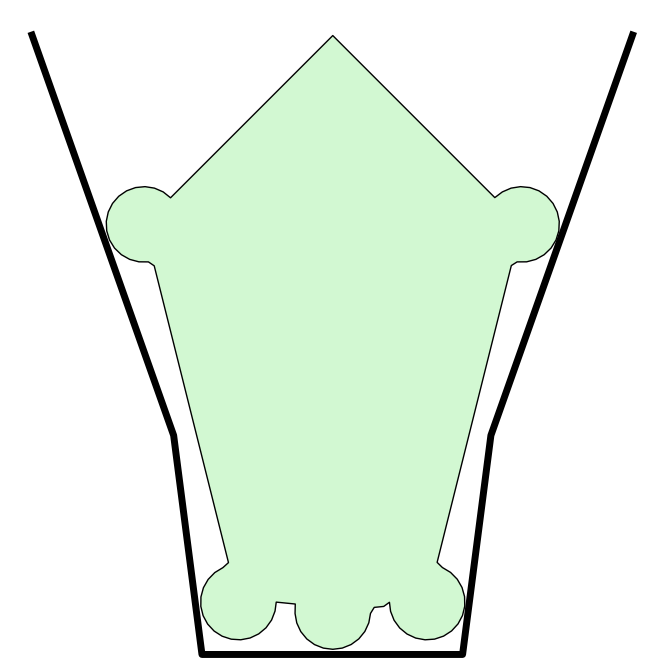
\includegraphics[width=1.5in]{figures/five_contact.png}
\end{center}
\caption{A peg-and-hole joint design, with five designed contacts between the peg and the hole. }
\label{fig:five_contact}
\end{figure}

Of course, for engineering purpose, the transition between the two stages of the hole joint should be curved rather than straight line, to avoid unclear normal directions. The bump near each contact should also be smaller, to eliminate unclear contacting point situation. This multistage hole joint can also help with insertion, as the initial insertion is easier because the joint is wider. As the peg gets deeper inside the hole, the majority of the peg is in place, and the hole becomes narrower to provide stability. 

If external forces is applied to the peg, with the manufacturing error, the peg should rotate around one of its side contacts, depending on how much error occurs near each contact point. However, such rotation can be small due to the length of the peg, which should be as long as one can allow. The actual length of the peg is also limited by the material and further assembly design. Further, we need to make sure that the peg is not easily breakable due to the length. 


\section{Comparison to other designs}

Given the design shown above with five contact points between the peg and the hole, we built the peg and the hole for testing to see if the assumptions are reasonable and the analysis are sound. We used a polyjet prototype machine to print the planar version of the peg and hole joints for testing, comparison, and analysis. The prototyping machine have a precision of 28 microns, the error would be small in this case for both joints. Therefore, to simulate a uniform error, which is our assumption made in above analysis, we built a uniformly larger hole joint compared to the design. Together with the joints that are built according to design, we tested how the pegs may potentially move inside the holes. To further illustrate the soundness of the design, we also designed pegs with three or four point contacts with the hole, as well as a peg with surface contacts with the hole. These peg joints, in theory, should all be stable inside the hole if no error is present. In Figure~\ref{fig:no_error}, we show the pegs inserted into the hole joint that is built with no error. 

\begin{figure*}
\begin{center}
\begin{subfigure}[t]{0.24\textwidth}
\begin{center}
\includegraphics[height=1.3in]{figures/five_point_no_error.jpg}
\end{center}
\label{fig:five_point_no_error}
\caption{Peg designed to contact hole with five points inserted into hole built with no error. }
\end{subfigure}
\begin{subfigure}[t]{0.24\textwidth}
\begin{center}
\includegraphics[height=1.3in]{figures/surface_no_error.jpg}
\end{center}
\label{fig:surface_point_no_error}
\caption{Peg designed to contact hole with all surfaces inserted into hole built with no error. }
\end{subfigure}
\begin{subfigure}[t]{0.24\textwidth}
\begin{center}
\includegraphics[height=1.3in]{figures/three_point_no_error.jpg}
\end{center}
\label{fig:three_point_no_error}
\caption{Peg designed to contact hole with three points inserted into hole built with no error. }
\end{subfigure}
\begin{subfigure}[t]{0.24\textwidth}
\begin{center}
\includegraphics[height=1.3in]{figures/four_point_no_error.jpg}
\end{center}
\label{fig:four_point_no_error}
\caption{Peg designed to contact hole with four points inserted into hole built with no error. }
\end{subfigure}
\end{center}
\label{fig:no_error}
\caption{Peg and hole joints of different types with no errors in the construction. }
\end{figure*}

Now, when no error is present in the hole, when inserted correctly, all pegs contact the hole joint at the designed locations. Translation along horizontal or vertical directions (viewing from top) is not possible with all these joints. 

There are, however, some issues with the peg designed to have surface contacts with the hole joint. As one can see in Figure~\ref{fig:surface_no_error}, the peg contacted the hole along multiple edges, but there are still visible separation between the edges closer to the base and the upper half of the hole joint, which were designed to contact. The cause is due to the tight contacts at the bottom half of the hole between the pegs and the hole, so that the hole joint is stretched, i.e., the peg is not fully inserted into the hole despite no visible space between the peg and the hole at the bottom. This is a common cause for polyjet prototyping parts, as the model are often printed with small defections, which results in materials {\em growing} slightly outside the designed solid regions, causing the joints to be over-fit or premature friction lock. This problem have to be addressed to allow assembly with multiple parts. In the past, similar issues were addressed by filling off the peg surfaces to allow fully insertion. Such filling, however, is not uniform, causing unpredictable surface shapes and contacts between pegs and hole. 

Such over-fit issue is much less observable with the pegs designed with point contacts. Even with the small defections near the contact points, due to the point contact in nature, the error does not accumulate as the surface contacts, which does not lead to over-fit or friction lock as easy. Therefore, this is one of the motivation for us to consider point contacts in practices. 

Even though translation inside the hole joints are not possible when no error is present in the hole joint, with the pegs design to contact the hole with three or four contacts, rotation motions are possible for the given design peg and external block size. The pegs cannot rotate around the contacts inside the hole, as the analysis show it would cause pinching, which is verified experimentally with these pegs as well. The issue raises when we use a point outside the peg-and-hole joint as the rotation center and rotates the peg block. In this situation, the pinching will not happen because of the different rotation centers, and the visible air-space between the peg and the hole, particularly near the transition point of the hole joint, allow the rotation to take place. In practice, with block that extends further outside the peg and hole joints, the rotations are less likely to happen due to the distance between the possible rotation center and the joints, but it is still one potential cause for concern. There are other issues with the pegs with three or four designed contact points, which we will analyze in the following sections. 

With the designed five contacts peg, however, the rotation is not possible even when we attempt to use an external point as rotation center. The two contacts near the bottom of the hole prevents any rotation  when no error is present. 



\begin{figure*}
\begin{center}
\begin{subfigure}[t]{0.24\textwidth}
\begin{center}
\includegraphics[height=1.3in]{figures/five_point_max_rotate.jpg}
\end{center}
\label{fig:five_point_max_rotate}
\caption{Peg designed to contact hole with five points inserted into hole built with uniform error, rotating at a maximum angle. }
\end{subfigure}
\begin{subfigure}[t]{0.24\textwidth}
\begin{center}
\includegraphics[height=1.3in]{figures/surface_max_rotate.jpg}
\end{center}
\label{fig:surface_point_max_rotate}
\caption{Peg designed to contact hole with surfaces inserted into hole built with uniform error, rotating at a maximum angle.  }
\end{subfigure}
\begin{subfigure}[t]{0.24\textwidth}
\begin{center}
\includegraphics[height=1.3in]{figures/three_point_max_rotate.jpg}
\end{center}
\label{fig:three_point_max_rotate}
\caption{Peg designed to contact hole with three points inserted into hole built with uniform error, rotating at a maximum angle.  }
\end{subfigure}
\begin{subfigure}[t]{0.24\textwidth}
\begin{center}
\includegraphics[height=1.3in]{figures/four_point_max_rotate.jpg}
\end{center}
\label{fig:four_point_max_rotate}
\caption{Peg designed to contact hole with four points inserted into hole built with uniform error, rotating at a maximum angle. }
\end{subfigure}
\end{center}
\label{fig:hole_error}
\caption{Peg and hole joints of different types with uniform errors in the construction. }
\end{figure*}

When we used the hole that are built with a uniform error (about 2 mm uniformly), rotation is possible, but the scale is quite different with these different designs. Figure~\ref{fig:hole_error} shows the same pegs inserted in the hole with errors, rotating at a maximum angle. As one can see, the proposed design with five contacts have the smallest possible rotation angle, which is roughly the same as the designed surface contacts. The peg designed with three point contacts have the largest possible rotation, followed by the peg with four designed contact points. 

The analysis leads to the following hypothesis, that the distance between the contacts (near the bottom of the peg) and the hole determines the possible rotations in a hole-joint with errors. The hypothesis can be supported by geometric analysis, showing that when the rotation center is near the top of the hole, the smaller the distance between the tip of the peg and the side edges near the bottom of the hole, the smaller the rotation can be. Therefore, to prevent rotations, we need to put contacts near the tip the peg with the side edges near the bottom of the hole, which is part of our proposed five-contact design. One possible other good design is to have only three contacts, but all three contacts are located near the tip of the peg, i.e. removing the two contacts in our proposed design near the bottom of the peg (top of the hole). This, however, would lead to further translation near the top of the hole with the same rotation, which would in turn allow further rotation near the bottom of the hole due to a further shift of rotation center. 

From the above simple comparison, we can see that our assumptions and analysis are both reasonable. We will further dive into the differences in different designs, to show that our proposed design can potentially lead to the best stability after insertion, and allow easy insertions as well. 


\subsection{Compared to three contacts with the hole}

First, we will take a closer look at pegs designed to contact with the hole at three points. These three points are placed like an isosceles triangle on the peg. We will further analyze the case where the contacts are allocated in a non-symmetric fashion in a later section. 

As discussed above, to prevent possible rotations of pegs inside the hole, especially when errors are present, one would like to put the contacts as close to the bottom of the hole as possible. Among all the designs with three contacts between the peg and the hole, this design would allow the least amount of rotation when inserted into a hole when errors are presented. 

Now, when compared to the proposed design of five contacts between the pegs and the holes, the proposed three contacts share the same design for half of the peg near the tip, while removing the two contacts between the peg and the whole near the base of the peg. Let us first consider the case when there is no error in the manufacturing process. 

When there is no error, given that the tilt angle of side walls of the hole is small compared to the length of the peg based on the analysis shown in the previous section, the three contacts should be sufficient to maintain the stability of the peg inside the hole joint. Any rotation of the contacts would lead to a pinch situation, so that no rotation of the peg inside the hole should be possible. However, in practice, due to the fact that the material may not be rigid enough to prevent instantaneous motion of the peg, and the contact area is small enough to be considered as points, a tilt angle smaller than the theoretical bound may still allow rotation of the peg. Such rotation, however, is prevented if additional contacts are present closer to the base of the peg compared to the two points contacting the side of the hole near the bottom. Therefore, three contacts may not be sufficient to prevent motion even when the manufacturing is perfect. 


When the error is present, things may become even worse with only three contacts. Since there exist errors, not all designed contacts can maintain their contact with the hole joint. Apart from the translations, the rotation can happen without causing pinch or pinch-like scenarios. Because the possibility of rotation, how large can the peg rotate is determined by where is the rotation center. Because there are only three contacts near the tip of the peg, given the same rotation angle permitted by the five-contact design proposed in this work, because there are no contacts near the base of the peg, the peg can then be translated towards the rotation center location, thus creating new space between the peg and the hole near the tip of the peg on the opposite side, which leads to more rotation. Therefore, a peg with only three contacts can always be rotated more compared to the proposed five contact design. Thus, the peg is less stable when inserted. 


\subsection{Compared to other five contacts with the hole}


Compared to other designs of the peg with five contacts, our design plans the contact between the peg and the side of the hole joint at two pairs of symmetric points, one pair near the tip of the peg, one near the base of the peg. We will show that this design would be more stable compared to the same number of contacts design at any other locations. 

First, let us consider the pair of contacts near the tip of the peg. This pair of contacts provides stability when error is present. Because the rotation center is at or beyond the base of the peg, the further the contact is from the rotation center, the faster it moves given the same rotation angle around the rotation center. Therefore, the closer this pair of contacts to the tip of the peg, the smaller the permitted rotation given the same amount of error. 

Second, let us consider the pair of contacts near the base. This pair of contacts provides stability when no error is present, but as long as they exist and closer to the base of the peg compared to the previously mentioned pair of contacts, which is always true as the other pair is furthest away from the base of the peg. This pair of contacts also participate in the decision of location of the rotation center when errors exist. 

If we do not consider the existence of the block outside the peg and the hole, the location of the contact is the rotation center. As analyzed above, the faster the contacts near the tip of the peg touch the hole, the smaller the permitted rotation is for a given error. The speed the pair of contacts moves is determined by the distance of that pair of contacts to the rotation center, therefore, this pair of contact should be as close to the base as possible to permit the smallest amount of rotation. 

If we take into account the external block beyond the peg and the hole, based on the amount of error in the manufacturing process, eventually the rotation center may need to be relocated to a point outside the peg and the hole. With the existence of the block external to the peg and hole, any rotation permitted must also not allow block to penetrate each other, as the basic property of rigid objects. Therefore, to allow maximum rotation, one the pair of contacts not near the tip of the peg must maintain contact with the hole as well as the external rotation center. This means the further this pair of contact is away from the base of the peg, further it slides towards the top of the hole to maintain contact. If the side-wall of the hole is tilted, which is in our design for easy insertion, the further the distance it is between the contact near the tip of the peg and the hole. Therefore, the larger the peg can rotate. 

Therefore, combining the above analysis, the design to put two pair of contacts as proposed, one near the tip of the peg, one near the bottom of the peg, is most stable with or without errors compared to all other possible designs that allows four contacts between the peg and the sidewall of the hole. The additional contact near the tip is placed to avoid pinching situation when inserting as analyzed in previous sections. So, our proposed design is superior to other designs with five contacts. 


\subsection{Compared to surface and non-symmetric contacts with the hole}

Now, given our proposed design of five contacts, we will further show that more contact would not improve stability. Also, we will show in this section that the surface contacts though is equivalent in analysis, would suffer more from errors in practice, again with or without errors. Also, non-symmetric placement of contacts on the side of the hole is not reasonable. 

First, compared with more contacts, translation would not be reduced regardless of how many more planned contacts we add. The rotation, however, is bounded by the pair of contacts closest to the tip and the base of the peg, as analyzed above. Therefore, more contacts would help reduce rotation either. 

Compared with surface contacts, the proposed design would provide the same amount of stability as the peg designed with surface contacts along all the walls of the hole joint. The challenge, however, is that in practice, the surface contacts may introduce additional problems. First, when no error is present, the surface contacts may suffer from manufacturing process that was shown in Figure~\ref{fig:surface_point_no_error} where the peg over-fill the hole joint. When error do exist, however, the contacts may not be the same as what we proposed in the five-point contact design, especially with non-uniform errors. When error is uniform, the situation would be the same as our proposed design. But when error are introduced by manual filling to over come the over-filling issue, they are usually non-uniform. 

When error is not uniform, the contacts may be non-symmetric, and may also be located at unpredictable locations. When the new candidate contacts are not near the tip and bottom of the peg, the resulting design would permit larger rotation, especially when the number of candidate contacts are smaller than four. On the other hand, the candidate contacts may further be non symmetric, one of the most extreme case would be shown in Figure~\ref{fig:uneven_max_rotate}. 

\begin{figure}
\begin{center}
\includegraphics[height=1.3in]{figures/uneven_max_rotate.jpg}
\end{center}
\label{fig:uneven_max_rotate}
\caption{Uneven contacts along the sidewall of the hole joint, rotating at a maximum angle. }
\end{figure}

When the contacts are non-symmetric, the largest rotation appears when the peg rotates around a point on the side that has no candidate contact near base, and at the same time the other side presents no candidate contacts near the tip of the peg. Figure~\ref{fig:uneven_max_rotate} illustrate such an example. In this case, the peg can rotate at a very large angle, compared to what permitted by the five-contact design proposed. 

With the proposed five-contact design, the error can also be non-symmetric. One important question is that whether the stability is still good when non-symmetric error exist. In above section, we said that we will design the bumps (planned contacts) larger than the known manufacturing error, whether uniform or non-uniform. This would mean that even when the non-uniform errors are introduced, the bumps would still remain candidate contacts, thus validating our previous analysis. 

\subsection{Hole with single or multiple stages}


The previous analysis and comparison would hold no matter how many {\em stages} the hole have. The multistage of the hole is introduced to help the insertion process. A single stage hole design would need to be tilted at a larger angle to allow error during the insertion process, especially the initial insert displacement. However, a smaller tilt angle would be preferred to provide stability and reduce possible rotations when errors exist, especially near the bottom of the hole. 

Due to these contradicting requirements, the hole is designed with multiple stages. The next logical question is, whether more stages make sense. Since the goal is to insert the peg into the bottom of the hole, and no stalemate should occur during the insertion process even when the inserting angle is wrong. Therefore, the maximum tilt angle would need to be smaller than the analyzed amount shown in previous section. The minimum tilting angle near the bottom of the hole should be as small as possible, to provide stability. Therefore, all intermediate stages, if exist, would be transitioning between the two extreme. However, since the most tolerant section is near the top of the hole to allow easy insertion, and no stalemate exist even with the largest tilt angle, the multiple stages would not provide additional stability or security during insertion, especially when there are no designed contacts in those stages. 

Putting all together, given a possible error of $\epsilon$, our proposed design is theoretically better than other designs to provide stability and ease of insertion. What is more, the proposed design not only applies to just peg-and-hole joints. The analysis holds for any joint type that is insertion based. 

\section{A generic automated design process for joints}
\label{sec:design}
Though the insights and the analysis shown above are generic to any insertion based joints, there are details of the design that has not been specified, such as the length of the peg relative the width and the tilt angle of the walls of the hole joint, etc. What is more, the insertion direction maybe outside the plane on which other motions are possible, which invalidates some of the analysis shown above.

Therefore, we will introduce an automated design process that can be used to generate a good design based on the designed relations between blocks. The goal for the design is to provide the most stability after the insertion, as well as providing ease of insertion when error exists in the insertion directions and block locations. 

As discussed above, usually the stability and the ease of insertion are two competing conditions, which we will further show in the proposed design process. We will present the process used to provide stability and ease of insertion separately at first, and then combine the result to balance between the two competing conditions to provide the most suitable design overall. Again, we will consider designed point contacts rather than surface contacts. 

\subsection{Stability design}


To make the joint as stable as possible, given the set of constraints provided by the socket, the possible motions allowed for the peg should be limited to a minimum. For simplicity, we will first study the socket-joint design on a plane, and consider the socket with only linear edges. 

If a 3D joint that is symmetric, then analyzing a projection of the socket-joint relation on a plane should be sufficient to bound the motion in all dimensions. If the 3D joint is not symmetric, the possible motion of the joint is also upper bounded by the least constraint intersection plane with the joint. Therefore, we study the joint design first on the plane. The planar constraint will be removed later. 

The assumption of linear edges is included for the simplicity of the analysis and the optimization for the design. A complex curve is hard to parameterize, thus is difficult to optimize the joint design under such constraints. Simpler curves is possible to be adapted while still maintaining the simplicity of the optimization process. However, it is possible to use many short linear edges to approximate a curve, and study the stability. Therefore, we start setting up the problem with linear edges. 


Let us consider the following parameterization of the problem. Given a socket with $n$ vertices connected by linear edges, let the $i$th planar vertex be denoted as $v^s_i = (x^s_i, y^s_i)$. Given a joint centered at $(x_0, y_0)$, and $m$ designed contacts with the socket, denote the $i$th designed contact location in the joint frame as $c_i = (x^p_i, y^p_i)$, where the joint frame is centered at $(x_0, y_0)$ and oriented at angle $\theta$ in the world frame in which the socket vertices are defined. Therefore, we can derive a transformation matrix $T$ that transforms the locations of the designed contacts from the joint frame to the world frame. We have, 

\begin{eqnarray}
T(x_0, y_0, \theta) = \begin{bmatrix}
\cos\theta & -\sin\theta & x_0\\
\sin\theta & \cos\theta & y_0 \\
0 & 0 & 1
\end{bmatrix}
\end{eqnarray}


The goal then is to minimize the largest possible angle $\theta$ so that the joint is not penetrating the socket. Let the $n$ points on the sockets are labeled counter clockwise, so that to have all the points inside the socket, they are on the left side of each line. Also, denote the location of the designed contacts of the peg in the world frame to be $^wc_i = (^wx^p_i, ^wy^p_i)$, which can be computed as
\begin{eqnarray}
\begin{bmatrix}
^wx^p_i\\ ^wy^p_i\\ 1
\end{bmatrix} = T(x_0, y_0, \theta) \cdot\begin{bmatrix}
x^p_i\\ y^p_i\\ 1
\end{bmatrix}
\end{eqnarray}

Therefore, putting all things together, we have the following optimization objective. 
\begin{eqnarray}
\min\max&\theta\\
\mathrm{subject\ to: } & \nonumber\\
(x^s_{k}-x^s_{j})&*&(^wy^p_i-y^s_{j})\nonumber\\
 - (y^s_{k}-y^s_{j})&*&(^wx^p_i-x^s_{j}) \geq 0 \\
\forall i\in m, j\in n&,& k=(j+1\mod n)\nonumber
\end{eqnarray}

Given the above objective function and the constraints, we know that to satisfy the constraints, each possible $\theta$ must put all contacts on the inside of the socket. To minimize the maximum possible $\theta$ that satisfy the constraints, we can find the best design. 

The given optimization, however, cannot be solved unless we specify the $n$ vertices of the socket. One way to solve the given process is to loop over possible locations of the socket, and compare all the best $\theta$ angles for each of the socket design, and choose the one with the minimum $\theta$. However, as the location of the vertices of the socket is not a finite choice, the process can take a long time to find an approximate optimal design. 

Another way to try to solve the given system is to alternate the variable set between the $n$ socket points and $m$ designed contacts. We first find the best location of the designed contacts assuming the location of the vertices of the sockets are known. Then, based on the designed contact locations in the joint frame, which we assume is known based on the results of the previous optimization process, and then compute the best socket vertices locations of this set of contacts. The process iterate until the $\theta$ cannot be reduced. This approach, however, may get stuck in the local minimum as the possible motion of $\theta$ may not be monotonic with respect to the socket and joint design. 

Another big issue is that given the above formation, to allow the smallest possible rotation angle $\theta$, the contacts should immobilize the joint inside the socket. However, this can be guaranteed for any immobilizing grasp, when no error is present. The stability we want is under an uniform error. Therefore, the above constraints should be updated to the following relation:
\begin{eqnarray}
(x^e_{k}-x^e_{j})&*&(^wy^p_i-y^e_{j})\nonumber\\
 - (y^e_{k}-y^e_{j})&*&(^wx^p_i-x^e_{j}) \geq 0 \\
\forall i\in m, j\in n&,& k=(j+1\mod n)\nonumber
\end{eqnarray}
where $x^e_i$ and $y^e_i$ should be the projection of $x^s_i$ and $y^s_i$ outwards for a distance of $\epsilon$, where $\epsilon$ is the uniform error that we may encounter in the manufacturing process. Another way to describe the relation between $v^s_i$ and $v^e_i$ is that for every $j\in n$ and $k = (j+1\mod n)$, we have 
\begin{eqnarray}
\overrightarrow{v^s_jv^s_k} \parallelsum\overrightarrow{v^e_jv^e_k}\\
d_{\parallelsum}(\overrightarrow{v^s_jv^s_k}, \overrightarrow{v^e_jv^e_k}) = \epsilon
\end{eqnarray}
where $d_{\parallelsum}(\cdot, \cdot)$ means the shortest distance between two parallel line segments. To guarantee the joints does not expand when there are errors in the socket, we also need to make sure that the contacts are made when there is no error with the socket, and define the given rotation angle $\theta$ to be $0$. Denote the locations of the designed contacts of the joints with the socket in the world frame as $^wc^{p(0)}_i = (^wx^{p(0)}_i, ^wy^{p(0)}_i)$, indicating that the rotation angle $\theta$ is $0$. Also, since $\theta$ can rotate to both directions symmetrically, the objective will also need to involve the absolute value of $\theta$. 

Therefore, putting all together, we will have the following objective, 
\begin{eqnarray}
\min\max&|\theta|\\
\mathrm{subject\ to: } & \nonumber\\
(x^s_{k}-x^s_{j})&*&(^wy^{p(0)}_i-y^s_{j})\nonumber\\
 - (y^s_{k}-y^s_{j})&*&(^wx^{p(0)}_i-x^s_{j}) \geq 0 \\
\forall i\in m, j\in n&,& k=(j+1\mod n)\nonumber\\
(x^e_{k}-x^e_{j})&*&(^wy^p_i-y^e_{j})\nonumber\\
 - (y^e_{k}-y^e_{j})&*&(^wx^p_i-x^e_{j}) \geq 0 \\
\forall i\in m, j\in n&,& k=(j+1\mod n)\nonumber\\
A \leq &y^s_j&\leq B\\
\mathrm{where}\\
\overrightarrow{v^s_jv^s_k} &\parallelsum&\overrightarrow{v^e_jv^e_k}\\
d_{\parallelsum}(\overrightarrow{v^s_jv^s_k}&,& \overrightarrow{v^e_jv^e_k}) = \epsilon
\end{eqnarray}

Then, solving the above optimization iteratively should be able to reach a best design locally. One can start the optimization from different initial socket design to get over the local extreme values. The constraint of $A \leq y^s_j\leq B$ is used to limit the total depth of the socket, so it cannot be infinitely deep, as we know from intuition, the longer and thiner the socket is, the smaller the possible motion is given a fixed error of $\epsilon$. Here, both $A$ and $B$ are given constants based on the size of the block that will utilize the joint designs. 

Considering the transition step of optimizing the location of the contact points and the socket vertices. Once we fix the location of the designed contacts on the joint, and attempts to adjust the socket vertices locations, we know from intuition that narrowing the tilt angle of the socket wall towards vertical would reduce the possible motion, and a incline of the socket edges may even further constraint the rotation angle $\theta$. However, there may exist other constraints that prevents the socket wall to tilt in such direction. For example, in a peg-and-hole joint design, the socket cannot be inclined because that would prevent the insertion of the peg that would achieve minimum rotation generated from the above design process. Therefore, given the additional constraints of the joint, we need to add appropriate constraints to the above formation. 

The above constraints are linear with respect to the location of the design contacts on the joint, which is the result of choosing linear edges on the socket design, making it possible to write the gradient analytically to improve the optimization process and step-out of the local extremes without using random based approaches. The alternative step of computing the vertex locations, however, is not linear, thus cannot be computed analytically. 


The proposed optimization methods though complete, is pure brute force. One may wish to find better, faster, and more intelligent approach to find the best socket design. Is it possible to find the design faster without relying on an optimization process, which is numerical at least partially in the above process. 



\subsection{Insertion design}

To guarantee the ease of insertion in the joint design, the process we need to take is a bit different from the above stability analysis. Instead of a discrete set of poses that we need to analyze and limit the possible poses, we are looking at a whole process of insertion. What is more, the definition of ease of insertion can be interpreted in many ways, so that we need to be careful in choosing the parameterization and the formation of the problem. 

Again, the analysis of the ease of insertion only makes sense under the existence of the errors. Here in the insertion process, however, in addition to the manufacturing error, it is the insertion location and direction error that we need to worry about. Therefore, an ease of insertion may be defined to be the design that allows the most amount of error in the insertion direction and block location. In this analysis, let us first assume that the insertion force direction is always along the orientation of the joint frame, which is reasonable under the assumption that the grasp of the blocks have no error. To account for the grasping error, however, the insertion force then can be within a small cone along the joint frame. We will further relax the constraint to allow the insertion direction error later. 

The success of insertion depends on two things. One, during the insertion process, the component of force pushing the joint into the socket should always be larger than the resistant force, such as friction. Two, the joint should never reach a configuration where the joint is not yet fully inserted while no progress can be made given the limit on the force direction and magnitude. For example, a socket with a flat bottom can create such a deadlock condition when the joint tip is in the shape of a triangle. Geometrically, the peg is locked in the corner of the socket, while not all the designed contacts are made near the designed areas. 

For a perfect joint design, we would like the joint frame to reach the $0$ rotation angle even when there exist errors in the insertion direction, or even with grasping error. This means that given the insertion force and any configuration of the joint, we would like there to exist a component of force navigating the joint frame towards the $0$ rotation angle. Such relation is easier to derive if there is not grasping error, meaning that the insertion force is always along the insertion direction. Once the grasping error is introduced, the joint frame may only be pushed into $(-\sigma, \sigma)$ range where $\sigma$ is small. 

To satisfy the above constraints, we need to not only look at the geometric relations, but also the insertion force and its components with respect to the socket edges. This, however, requires us to know which edges of the socket the joint is making contacts with. In this process, we first choose to assume that the joint design is known, and adjust the socket vertex locations. 

Since again we are assuming the socket edges are linear, then the displacement of the block should not affect the force decomposition. Therefore, we again only need to consider the rotation in this case. To satisfy the first condition, we need to maximize the angle $\phi$ so that the force decomposition will always push the joint towards the bottom of the socket. We therefore can write the following objective given insertion force $F$ and friction coefficient $\mu$, let $\overrightarrow{A} = \overrightarrow{F\cos(\arctan2(y^p_i, x^p_i))}$, $\overrightarrow{B} = \overrightarrow{A}\cdot\overrightarrow{v^s_jv^s_k}$, and $\overrightarrow{C} = \overrightarrow{A\cos(\arcsin(B/A))}$, 

\begin{eqnarray}
\max &\phi&\\
\mathrm{subject\ to: }&&\nonumber\\
\sum(|\overrightarrow{B}| - \mu\cdot |\overrightarrow{C}|) &>& 0\\
\forall\mathrm{contact\ } i\mathrm{\ with\ edge}& v_jv_k&, k=(j+1\mod n).\nonumber 
\end{eqnarray}

This step, however, is very easy to satisfy, as we even know geometrically how to place these vertices on the socket. 

The second step, however, is to guarantee that for any $\phi$ that is greater than $0$, the gradient of $\phi$ should be towards $0$. The gradient of $\phi$ depends on time $t$, which has not shown up in the analysis above. The change of $\phi$, however, is based on the above relation between $\overrightarrow{B}$ and $\overrightarrow{C}$. We can define $\phi$ as the following, 
\begin{eqnarray}
\phi(t+1) - \phi(t) = \sum(|\overrightarrow{B}| - \mu\cdot |\overrightarrow{C}|)\\
\forall\mathrm{contact\ } i\mathrm{\ with\ edge} v_jv_k, k=(j+1\mod n)\nonumber
\end{eqnarray}

Then, to satisfy the second relation, we should maintain that $\phi\cdot\dot{\phi} < 0$, meaning that the $\phi$ should always move towards $0$. The angle $\phi$ now, is no longer the maximum angle allowed in insertion error, but the insertion angle along the insertion process. This means that this step needs to be separate from the above optimization process which maximize $\phi$. However, once a $\phi$ is computed, we will then test the above constraint to see if the condition is satisfied, to decide whether to accept or reject a design. 

Another possible criteria to optimize associated with the insertion process is the time it takes for the insertion. In other words, in the above definition of $\phi$ that is dependent on time, we want to minimize the total time it takes $\phi$ to reach $0$. Therefore, another possible formation is described as below, 

\begin{eqnarray}
\min T &\\
\mathrm{subject\ to: }&\nonumber\\
\phi(T) = 0&\\
\phi(t) - \phi(t-1) =& \sum(|\overrightarrow{B}| - \mu\cdot |\overrightarrow{C}|)\\
\forall\mathrm{contact\ } i\mathrm{\ with\ edge\ }& v_jv_k\\
k=(j+1\mod n),&\ t\leq T&\nonumber
\end{eqnarray}


\subsection{Putting pieces together}








\section{Applied in assembly}
\label{sec:exp}

\section{Conclusion and future work}

\renewcommand*{\bibfont}{\small}
\printbibliography

\end{document}
